\lstset{
	basicstyle=\ttfamily\footnotesize,
	keywordstyle=\color{blue},
	stringstyle=\color{red},
	commentstyle=\color{gray},
	numbers=left,
	numberstyle=\tiny,
	stepnumber=1,
	numbersep=10pt,
	frame=single,
	breaklines=true,
	captionpos=b,
	tabsize=4,
	showspaces=false,
	showstringspaces=false,
	language=Python
}

\chapter{The Experiments of Hand Pose Recognition}

\section{Hand Pose Data Training Preparation}
\subsection*{Function: \texttt{read\_landmarks}}

The \texttt{read\_landmarks} function is designed to extract hand pose landmarks from a dataset of labeled images using Mediapipe's \texttt{Hands} module. It processes all images in subdirectories corresponding to different labels, extracts features, and prepares the data for machine learning tasks.

\begin{lstlisting}[language=Python, caption=The \texttt{read\_landmarks} function]
def read_landmarks(dataset, labels):
	# Initialize Mediapipe Hands and Drawing
	hands = mp_hands.Hands(static_image_mode=False,
	max_num_hands=2,
	min_detection_confidence=0.5,
	min_tracking_confidence=0.5)
	
	kelas = np.eye(len(labels))
	y = []
	
	images_by_label = {}
	X = []
	for i, label in enumerate(labels):
		# Construct the directory path
		directory_path = os.path.join(dataset, label)
	
		# Check if the directory exists
		if not os.path.exists(directory_path):
			print(f"Directory '{directory_path}' does not exist.")
			images_by_label[label] = []
			continue
	
	# List all `.jpg` files in the directory
	filenames = [f for f in os.listdir(directory_path) if f.endswith('.jpg')]
	
	# Read images and store them as frames
	# frames = []
	for filename in filenames:
		file_path = os.path.join(directory_path, filename)
		frame = cv2.imread(file_path)  # Read the image with OpenCV
		fitur = feature_extract(frame, hands)
		X.append(fitur)
		y.append(kelas[i])
	
	hands.close()
	return np.array(X), np.array(y)
\end{lstlisting}

\subsection*{Explanation}

The \texttt{read\_landmarks} function performs the following key tasks:

\subsubsection*{1. Initialize Mediapipe Hands}
\begin{itemize}
	\item \texttt{static\_image\_mode=False}: Allows the function to dynamically process images or frames.
	\item \texttt{max\_num\_hands=2}: Configured to detect up to two hands in an image.
	\item \texttt{min\_detection\_confidence=0.5}: Sets the minimum confidence threshold for hand detection.
	\item \texttt{min\_tracking\_confidence=0.5}: Ensures reliable tracking of hand landmarks once detected.
\end{itemize}

\subsubsection*{2. One-Hot Encode Labels}
A one-hot encoded matrix (\texttt{kelas}) is created for the labels using:
\begin{lstlisting}[language=Python]
	kelas = np.eye(len(labels))
\end{lstlisting}
For example, if there are three labels:
\[
\begin{bmatrix}
	1 & 0 & 0 \\
	0 & 1 & 0 \\
	0 & 0 & 1 \\
\end{bmatrix}
\]
The list \texttt{y} is initialized to store the corresponding one-hot encoded labels for each image.

\subsubsection*{3. Process Each Label Directory}
The function iterates through the given labels:
\begin{lstlisting}[language=Python]
	for i, label in enumerate(labels):
	directory_path = os.path.join(dataset, label)
\end{lstlisting}
It constructs the full directory path for each label's subdirectory. If the directory does not exist, a warning is printed, and an empty list is assigned to that label.

\subsubsection*{4. Read and Process Images}
For each valid directory, the function lists all filenames ending with \texttt{.jpg}:
\begin{lstlisting}[language=Python]
	filenames = [f for f in os.listdir(directory_path) if f.endswith('.jpg')]
\end{lstlisting}
It then reads each image using OpenCV:
\begin{lstlisting}[language=Python]
	frame = cv2.imread(file_path)
\end{lstlisting}
Hand pose features are extracted using the \texttt{feature\_extract} function:
\begin{lstlisting}[language=Python]
	fitur = feature_extract(frame, hands)
\end{lstlisting}
The extracted features are appended to the \texttt{X} list, and the corresponding one-hot encoded label is added to the \texttt{y} list.

\subsubsection*{5. Close Mediapipe Resources and Return Data}
Once all images are processed, the Mediapipe \texttt{Hands} module is closed:
\begin{lstlisting}[language=Python]
	hands.close()
\end{lstlisting}
Finally, the function returns \texttt{X} (a NumPy array of extracted features) and \texttt{y} (a NumPy array of one-hot encoded labels).

\subsection*{Output}
\begin{itemize}
	\item \texttt{X}: A NumPy array containing the extracted hand pose features for all images.
	\item \texttt{y}: A NumPy array of one-hot encoded labels corresponding to each feature in \texttt{X}.
\end{itemize}

\subsection*{Practical Use Case}
The \texttt{read\_landmarks} function is particularly useful in preprocessing datasets for hand pose recognition tasks. By extracting and normalizing geometric features from images, it prepares the data for downstream machine learning models.


The function \texttt{read\_landmarks} is designed to process a dataset of hand pose images, extract features using Mediapipe, and prepare the data for machine learning models. Specifically, it:
\begin{enumerate}
	\item Traverses a dataset organized into subdirectories, where each subdirectory represents a label.
	\item Reads all \texttt{.jpg} images within each subdirectory.
	\item Extracts hand pose features from each image using Mediapipe's \texttt{Hands} module.
	\item Prepares feature data (\texttt{X}) and one-hot encoded labels (\texttt{y}) for training or testing a machine learning model.
\end{enumerate}

\subsection{Function Parameters}
\begin{itemize}
	\item \texttt{dataset (str)}: The root directory containing subdirectories, each corresponding to a label.
	\item \texttt{labels (list)}: A list of label names, where each label matches a subdirectory name within \texttt{dataset}.
\end{itemize}

\subsection*{Step 1: Initialize Mediapipe Hands}
The function initializes Mediapipe's \texttt{Hands} module to process the images:
\begin{itemize}
	\item \texttt{static\_image\_mode=False}: Operates in dynamic mode for handling multiple frames or videos.
	\item \texttt{max\_num\_hands=2}: Configured to detect and process up to two hands per image.
	\item \texttt{min\_detection\_confidence=0.5}: Specifies the minimum confidence threshold for detecting a hand in an image.
	\item \texttt{min\_tracking\_confidence=0.5}: Specifies the minimum confidence required to track hand landmarks reliably.
\end{itemize}

\subsection*{Step 2: One-Hot Encode Labels}
\begin{lstlisting}[language=Python]
	kelas = np.eye(len(labels))
	y = []
\end{lstlisting}
A one-hot encoded matrix (\texttt{kelas}) is created for the labels. For instance, if there are three labels, the one-hot encoded representation would look like:
\[
\begin{bmatrix}
	1 & 0 & 0 \\
	0 & 1 & 0 \\
	0 & 0 & 1 \\
\end{bmatrix}
\]
The \texttt{y} list is initialized to store the labels corresponding to each image.

\subsection*{Step 3: Iterate Over Labels}
The function loops through each label and constructs the full directory path for each subdirectory:
\begin{lstlisting}[language=Python]
	for i, label in enumerate(labels):
	directory_path = os.path.join(dataset, label)
\end{lstlisting}

\subsection*{Step 4: List All \texttt{.jpg} Files}
To retrieve all the image files within each subdirectory, the function uses:
\begin{lstlisting}[language=Python]
	filenames = [f for f in os.listdir(directory_path) if f.endswith('.jpg')]
\end{lstlisting}
This collects only filenames with a \texttt{.jpg} extension from the directory.

\subsection*{Step 5: Read and Process Images}
The function processes each image file in the directory:
\begin{lstlisting}[language=Python]
	for filename in filenames:
	file_path = os.path.join(directory_path, filename)
	frame = cv2.imread(file_path)
	fitur = ekstraksi_fitur(frame, hands)
	X.append(fitur)
	y.append(kelas[i])
\end{lstlisting}
For every image:
\begin{enumerate}
	\item The full file path is constructed using \texttt{os.path.join}.
	\item The image is read using OpenCV's \texttt{cv2.imread}.
	\item The \texttt{ekstraksi\_fitur} function is called to extract hand pose features from the image using Mediapipe.
	\item The function normalizes hand landmarks for left and right hands.
	\item The extracted features are appended to \texttt{X}, and the corresponding one-hot encoded label is appended to \texttt{y}.
\end{enumerate}

\subsection*{Output}
The function returns the following:
\begin{itemize}
	\item \texttt{X}: A NumPy array containing the extracted features for all images in the dataset.
	\item \texttt{y}: A NumPy array of one-hot encoded labels corresponding to each set of features in \texttt{X}.
\end{itemize}

\subsection*{Purpose of Concatenating Hand Features}
In the feature extraction step, landmarks from both the left and right hands are concatenated into a single vector. This unified representation captures spatial relationships between the hands, enabling the model to understand interactions between the two hands (e.g., in sign language or complex gestures). If only one hand is detected, the unused hand’s feature vector is set to zeros, ensuring consistency in the feature size. This approach simplifies model training and ensures robustness in handling frames with varying numbers of detected hands.

\subsection*{Example Usage of \texttt{read\_landmarks}}
The following example demonstrates how to use the \texttt{read\_landmarks} function to prepare a dataset for training and testing a machine learning model. It includes the steps for defining the dataset and labels, calling the function, and splitting the data into training and testing sets.

\begin{lstlisting}[language=Python, caption=Example Usage of \texttt{read\_landmarks}]
	# Example usage
	dataset = "../dataset"                  # Base dataset directory
	labels = ["One", "Two", "Three"]        # List of labels (subdirectories)
	
	# Call the function
	X, y = read_landmarks(dataset, labels)
	X_train, X_test, y_train, y_test = train_test_split(X, y, test_size=0.2, random_state=40)
	print(X_train.shape, y_train.shape, X_test.shape, y_test.shape)
\end{lstlisting}

\subsection*{Explanation}
\begin{itemize}
	\item \texttt{dataset}: Specifies the base directory containing the dataset. Each label should have a corresponding subdirectory in this path containing the images for that label.
	\item \texttt{labels}: A list of subdirectory names representing the classes (e.g., "One", "Two", "Three"). Each label corresponds to a unique class in the dataset.
\end{itemize}

The \texttt{read\_landmarks} function is called with the dataset directory and the list of labels as arguments. It returns two outputs:
\begin{itemize}
	\item \texttt{X}: A NumPy array containing the extracted features for all images in the dataset.
	\item \texttt{y}: A NumPy array containing the one-hot encoded labels for each image.
\end{itemize}

The dataset is then split into training and testing subsets using \texttt{train\_test\_split}, a function from the \texttt{sklearn.model\_selection} module. The arguments are as follows:
\begin{itemize}
	\item \texttt{test\_size=0.2}: Specifies that 20\% of the data is reserved for testing.
	\item \texttt{random\_state=40}: Ensures reproducibility by fixing the random seed.
\end{itemize}

Finally, the shapes of the resulting datasets are printed:
\begin{itemize}
	\item \texttt{X\_train.shape}: The shape of the training feature set.
	\item \texttt{y\_train.shape}: The shape of the training label set.
	\item \texttt{X\_test.shape}: The shape of the testing feature set.
	\item \texttt{y\_test.shape}: The shape of the testing label set.
\end{itemize}

This example shows how to preprocess the dataset and prepare it for use in a machine learning workflow.

\section{Model Training and Evaluation}

The following code demonstrates the process of configuring, training, and evaluating a machine learning model for hand pose recognition. It includes the initialization of hyperparameters, model creation, compilation, training, evaluation, and saving.

\begin{lstlisting}[language=Python, caption=Model Training and Evaluation]
	# Parameters
	input_size = X_train.shape[1]  # Number of features (flattened landmarks)
	num_classes = len(labels)      # Number of labels
	batch_size = 32                # Batch size for DataLoader
	learning_rate = 0.01           # Learning rate
	num_epochs = 200               # Number of epochs
	
	from keras.optimizers import SGD
	
	# Create model, loss function, and optimizer
	model = get_model(input_size=input_size, num_classes=num_classes)
	
	# Display the model summary
	model.summary()
	
	# Compile the model
	model.compile(optimizer=SGD(learning_rate=learning_rate),
	loss='categorical_crossentropy',
	metrics=['accuracy'])
	
	# Train the model
	history = model.fit(
		X_train, y_train,
		validation_split=0.2,
		epochs=num_epochs,
		batch_size=batch_size,
		verbose=1
	)
	
	# Evaluate the model
	test_loss, test_accuracy = model.evaluate(X_test, y_test, verbose=0)
	print(f"Test Accuracy: {test_accuracy:.2f} %")
	
	output_path = "outputs"
	model_name = "model.keras"
	if not os.path.exists(output_path):
		os.makedirs(output_path)  # Create directory if it doesn't exist
		print(f"Directory '{output_path}' created.")
	model.save(os.path.join(output_path, model_name))
\end{lstlisting}

\subsection*{Explanation}

The process is divided into multiple steps:

\subsubsection*{1. Define Hyperparameters}
\begin{itemize}
	\item \texttt{input\_size = X\_train.shape[1]}: Determines the number of input features, which corresponds to the number of flattened landmarks extracted from the dataset.
	\item \texttt{num\_classes = len(labels)}: Defines the total number of classes in the dataset based on the length of the \texttt{labels} list.
	\item \texttt{batch\_size = 32}: Specifies the number of samples to be processed in one training batch.
	\item \texttt{learning\_rate = 0.01}: Sets the learning rate for the optimizer, which controls the step size during weight updates.
	\item \texttt{num\_epochs = 200}: Specifies the number of complete passes through the training dataset.
\end{itemize}

\subsubsection*{2. Create and Compile the Model}
The model is created using the \texttt{get\_model} function, which takes the \texttt{input\_size} and \texttt{num\_classes} as parameters. The model summary is displayed using:
\begin{lstlisting}[language=Python]
	model.summary()
\end{lstlisting}
This provides a detailed view of the model’s architecture, including the number of layers, parameters, and input/output shapes.

The model is then compiled using the Stochastic Gradient Descent (SGD) optimizer:
\begin{lstlisting}[language=Python]
	model.compile(optimizer=SGD(learning_rate=learning_rate),
	loss='categorical_crossentropy',
	metrics=['accuracy'])
\end{lstlisting}
\begin{itemize}
	\item \texttt{SGD}: A simple optimizer that updates weights using gradients calculated from the loss function.
	\item \texttt{categorical\_crossentropy}: The loss function used for multi-class classification problems.
	\item \texttt{metrics=['accuracy']}: Specifies accuracy as the evaluation metric during training.
\end{itemize}

\subsubsection*{3. Train the Model}
The model is trained using the \texttt{fit} method:
\begin{lstlisting}[language=Python]
	history = model.fit(
		X_train, y_train,
		validation_split=0.2,
		epochs=num_epochs,
		batch_size=batch_size,
		verbose=1
	)
\end{lstlisting}
\begin{itemize}
	\item \texttt{X\_train, y\_train}: The training data and corresponding labels.
	\item \texttt{validation\_split=0.2}: Reserves 20\% of the training data for validation.
	\item \texttt{epochs=num\_epochs}: The model is trained for the specified number of epochs.
	\item \texttt{batch\_size=batch\_size}: Processes samples in batches of size 32.
	\item \texttt{verbose=1}: Enables detailed logging of the training progress.
\end{itemize}

\subsubsection*{4. Evaluate the Model}
The trained model is evaluated on the test dataset using:
\begin{lstlisting}[language=Python]
	test_loss, test_accuracy = model.evaluate(X_test, y_test, verbose=0)
\end{lstlisting}
The test loss and accuracy are calculated, and the accuracy is printed:
\begin{lstlisting}[language=Python]
	print(f"Test Accuracy: {test_accuracy:.2f} %")
\end{lstlisting}

\subsubsection*{5. Save the Model}
The trained model is saved to a directory:
\begin{lstlisting}[language=Python]
if not os.path.exists(output_path):
	os.makedirs(output_path) 

model.save(os.path.join(output_path, model_name))
\end{lstlisting}
\begin{itemize}
	\item \texttt{output\_path}: The directory where the model will be saved.
	\item \texttt{model\_name}: The name of the saved model file.
	\item \texttt{os.makedirs}: Ensures that the directory is created if it does not already exist.
\end{itemize}

\subsection*{Practical Use Case}
This process is designed for training and evaluating a deep learning model for hand pose recognition. The hyperparameters can be adjusted based on the complexity of the dataset, and the model can be reused for predictions by loading the saved file.


\section{Inference Results of Hand Pose Classification}

\begin{figure}[h]
	\centering
	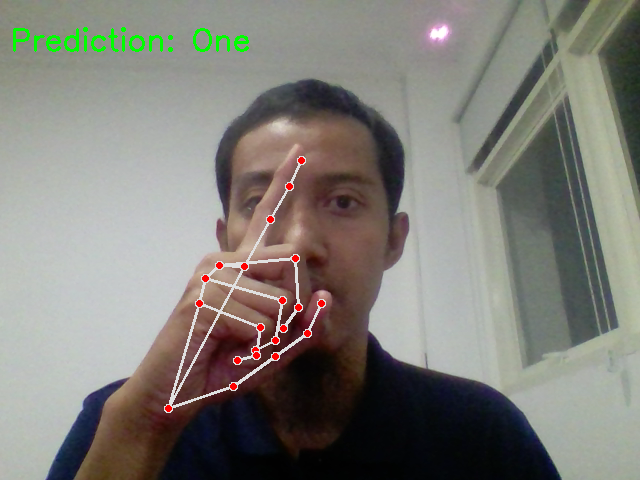
\includegraphics[width=0.33\linewidth]{img/1} 
	
\includegraphics[width=0.33\linewidth]{img/2}
	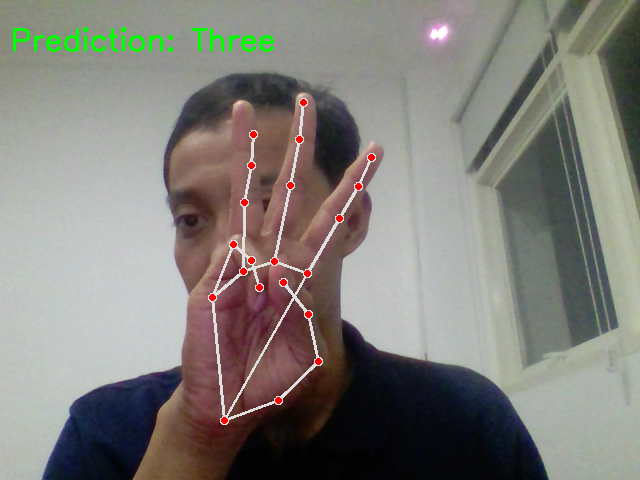
\includegraphics[width=0.32\linewidth]{img/3}
	\caption{Inference of hand pose classification}
	\label{fig:model_inference} % Reference the figure in your text using \ref{fig:unique_label}
\end{figure}
Figure \ref{fig:model_inference} illustrates the inference results of a TensorFlow-based hand pose classification model. The model successfully classifies hand poses into three distinct categories: "One," "Two," and "Three." Below is a detailed explanation of the components and insights derived from this result.

\subsubsection*{1. Visualization of Hand Landmarks}
The red dots and lines overlaying the hands represent the detected hand landmarks and their connections. These landmarks are extracted using a hand pose estimation framework, such as Mediapipe. Each hand is characterized by 21 key points corresponding to specific parts of the hand, including fingertips, knuckles, and the wrist. The skeletal structure formed by connecting these landmarks visually highlights the pose and is essential for feature extraction.

\subsubsection*{2. Hand Pose Classification}
The text above each image ("Prediction: One," "Prediction: Two," "Prediction: Three") displays the output of the classification model. This output is based on the features extracted from the hand landmarks and fed into the trained TensorFlow model. The model classifies the hand poses as follows:
\begin{itemize}
	\item \textbf{Left Image ("One")}: The model recognizes the pose where one finger is raised.
	\item \textbf{Middle Image ("Two")}: The model identifies the pose with two fingers raised.
	\item \textbf{Right Image ("Three")}: The model detects the pose with three fingers raised.
\end{itemize}
The predictions are shown in green text, indicating the model's confidence and clarity in its classification.

\subsubsection*{3. Context of the Images}
These images demonstrate a real-time application of the hand pose classification model. A person performs different hand gestures in front of a camera, and the model classifies each gesture in real-time. The inference process includes:
\begin{enumerate}
	\item Capturing frames from the camera.
	\item Detecting and extracting hand landmarks.
	\item Normalizing and preprocessing the extracted landmark features.
	\item Feeding the features into the trained classification model to predict the hand pose.
\end{enumerate}
The results are displayed by overlaying the predictions and skeletal hand landmarks onto the original images.

\subsubsection*{4. Application and Use Case}
This demonstration highlights the potential applications of the hand pose classification model, which include:
\begin{itemize}
	\item \textbf{Sign Language Recognition}: Translating hand gestures into text or speech for communication.
	\item \textbf{Human-Computer Interaction}: Enabling gesture-based control in devices or virtual environments.
	\item \textbf{Gaming}: Using hand gestures as inputs for gameplay mechanics.
	\item \textbf{Education and Training}: Assisting in teaching or monitoring hand poses in various activities.
\end{itemize}

\subsubsection*{5. Performance Indicators}
The consistent and accurate predictions in these images demonstrate the robustness and generalizability of the model across different hand poses. The quality of the skeletal overlay further indicates the effective use of hand landmark detection as a preprocessing step.





